\chapter{Applications of quantum phase estimation}\label{chap:app_qpe}

\section{Ground state energy estimation}\label{sec:groundenergy}

As an application, we use QPE to solve the problem of estimating the ground state energy of a Hamiltonian. 
Let $H$ be a Hermitian matrix with eigendecomposition
\begin{equation}
H\ket{\psi_j}=\lambda_j \ket{\psi_j}.
\end{equation}
Below are two examples of Hamiltonians commonly encountered in quantum many-body physics.
\begin{exam}[Transverse field Ising model]
The Hamiltonian for the one dimensional transverse field Ising model (TFIM) with nearest neighbor interaction of length $n$ is
\begin{equation}\label{eqn:ham_tfim}
H=-\sum_{i=1}^{n-1} Z_iZ_{i+1}-g\sum_{i=1}^n X_i.
\end{equation}
The dimension of the Hamiltonian matrix $H$ is $2^n$. 
\end{exam}

\begin{exam}[Fermionic system in second quantization]
\label{exam:fermion_hamiltonian}
For a fermionic system (such as electrons), the Hamiltonian can be expressed in terms of the creation and annihilation operators as
\begin{equation}
H=\sum_{ij=1}^{n} T_{ij} \hat{a}_{i}^{\dagger} \hat{a}_{j}+\sum_{ijkl=1}^{n} V_{ijkl} \hat{a}_i^{\dagger}\hat{a}_j^{\dagger}\hat{a}_l \hat{a}_k.
\label{eqn:fermion_hamiltonian}
\end{equation}
The creation and annihilation operators $\hat{a}^{\dag}_i,\hat{a}_i$ can be converted into Pauli operators via e.g. the Jordan-Wigner transform as
\begin{equation}
\hat{a}_{i}=Z^{\otimes (i-1)}\otimes\frac12(X+\I Y)\otimes I^{\otimes (N-i)}, \quad \hat{a}^{\dagger}_i=Z^{\otimes (i-1)}\otimes\frac12(X-\I Y)\otimes I^{\otimes (N-i)}.
\label{eqn:jordan_wigner}
\end{equation}
Here $X,Y,Z,I$ are single-qubit Pauli-matrices.  
The dimension of the Hamiltonian matrix $\hat{H}$ is thus $2^n$. 


The number operator takes the form
\begin{equation}
    \hat{n}_{i}:=\hat{a}^{\dag}_{i}\hat{a}_{i}=\frac12 (I-Z_{i}).
    \label{eq:ndecomp}
\end{equation}
For a given state $\ket{\Psi}$, the total number of particles is
\begin{equation}
N_e=\Braket{\Psi|\sum_{i=1}^n \hat{n}_i|\Psi}.
\end{equation}
The Hamiltonian $H$ preserves the total number of particles $N_e$.
\end{exam}

Without loss of generality we assume $0<\lambda_0\le\lambda_1\le \cdots  <\lambda_{N-1}<\frac12$. Note that for the purpose of estimating the ground state energy, we do not necessarily require a positive energy gap. 
For simplicity of the presentation, we still assume that the ground state is non-degenerate, i.e., $\lambda_0<\lambda_1$. 
We are also provided an approximate eigenstate
\begin{equation}
\ket{\phi}=\sum_{k\in[N]} c_k \ket{\psi_k},
\end{equation}
of which the overlap with the ground state is  $p_0=\abs{\braket{\phi|\psi_0}}^2$. Our goal is to estimate $\lambda_0$ to precision $\epsilon=2^{-d}$. We  assume $\epsilon<\lambda_0$. This appears in many problems in quantum many-body physics, quantum chemistry, optimization etc.

In order to use QPE (based on QFT), we assume access to the unitary evolution operator $U=e^{\I 2\pi H}$. This is called a Hamiltonian simulation problem, which will be discussed in detail in later chapters.
For now we assume $U$ can be implemented exactly.
Then
\begin{displaymath}
U\ket{\psi_0}=e^{\I 2\pi \lambda_0}\ket{\psi_0}.
\end{displaymath}
This becomes a phase estimation problem, where the input vector is not an exact eigenstate. 
Following the discussion in \cref{sec:analysis_qpe}, if \emph{all} eigenvalues $\lambda_j$ can be exactly represented by $d$-bit numbers, we obtain both the ground state and the ground state energy with probability $p_0$.
Therefore repeating the process for $\Or(p_0^{-1})$ times we obtain the ground state energy.

Now we relax both conditions (1) and (2) in \cref{sec:analysis_qpe}, and apply the QPE circuit in \cref{fig:circ_qpe_qft} to an initial state $\ket{0^t}\ket{\phi}$ for some $t>d$.
Similar to \cref{eqn:qpe_exactvec}, we have
\begin{equation}
\begin{split}
\ket{0^t}\ket{\phi} \xrightarrow{U_{\mathrm{FT}}\otimes I} & \sum_{k}c_k\frac{1}{\sqrt{T}}\sum_{j\in[T]}\ket{j}\ket{\psi_k}\\
\xrightarrow{\mc{U}} & \sum_{k} c_k \frac{1}{\sqrt{T}}\sum_{j\in[T]}\ket{j}U^j\ket{\psi_k}= \sum_{k} c_k \frac{1}{\sqrt{T}}\sum_{j\in[T]}\ket{j}e^{\I 2\pi \lambda_k j}\ket{\psi_k}\\
\xrightarrow{U_{\mathrm{FT}}^{\dag}\otimes I} &  
\sum_{k} c_k \sum_{k'\in[T]}\left(\frac{1}{T}\sum_{j\in[T]}
e^{\I 2\pi j\left(\lambda_k -\frac{k'}{T}\right)}\right)\ket{k'}\ket{\psi_k}\\
=& \sum_{k} \sum_{k'\in[T]} c_k \gamma_{k,k'}\ket{k'}\ket{\psi_k}.
\end{split}
\label{eqn:qpe_inexactvec}
\end{equation}
Here 
\begin{equation}
\gamma_{k,k'}=\frac{1}{T}\sum_{j\in[T]}
e^{\I 2\pi j\left(\lambda_k -\frac{k'}{T}\right)}=\frac{1}{T}\frac{1-e^{\I 2\pi T\left(\lambda_k - \wt{\varphi}_{k'}\right)}}{1-e^{\I 2\pi \left(\lambda_k - \wt{\varphi}_{k'}\right)}}, \quad \wt{\varphi}_{k'}=\frac{k'}{T}.
\end{equation}
Therefore the definition in \cref{eqn:gamma_0k} is a special case.



Our algorithm is simple: we would like to run QPE $M$ times, and denote the output of the $\ell$-th run by $\wt{\varphi}^{(\ell)}_{k'}$. 
Then we take the minimum of the measured output $\min_{\ell}\wt{\varphi}^{(\ell)}_{k'}$ as the estimate to the ground state energy.
The hope is to obtain the ground state energy to accuracy $\epsilon$ with success probability at least $1-\delta$ for any $\delta>0$. 
Let us now analyze this algorithm. 


If $\varphi_0$ has an exact $d$-bit representation, i.e., $\lambda_0=\wt{\varphi}_{k'_0}$ for some integer $k'_0$, then $\gamma_{k'_0,k'}=\delta_{k'_0,k'}$. 
It may seem that this implies with probability $p_0$, we obtain the exact estimate of $\varphi_0$, and correspondingly the eigenstate $\ket{\psi_0}$ is stored in the system register. This is much better than the previous assumption that \emph{all} eigenvalues $\lambda_j$ need to be represented by a $d$-bit number.

Unfortunately, this analysis is not correct.
In fact, for any $\lambda_k$ that does not have an exact $t$-bit representation (note that $t>d$), we may have $\gamma_{k,k''}\ne 0$ and $\wt{\varphi}_{k''}<\lambda_0$, i.e., we obtain an energy estimate that is lower than the ground state energy! Therefore the probability of ending up in the state $\ket{k''}\ket{\psi_k}$ is $\abs{c_k\gamma_{k,k''}}^2$, i.e., it is still possible to obtain a wrong ground state energy. This is called the \emph{aliasing effect}.

We demonstrate below that if $T$ is large enough, we can control the probability of underestimating the ground state energy. 
Since $\lambda_0$ is the ground state energy, and all eigenvalues are in $(0,1/2)$, when $\wt{\varphi}_{k'}\le \lambda_0-\epsilon$, we have 
\begin{equation}
\abs{\lambda_k-\wt{\varphi}_{k'}}_1\ge \abs{\lambda_0-\wt{\varphi}_{k'}}_1=\lambda_0-\wt{\varphi}_{k'}\ge \epsilon, \quad \forall k\in[N].
\end{equation}
Then the probability of under estimating the ground state energy by $\epsilon$ is
\begin{equation}
\begin{split}
P(\wt{\varphi}_{k'}\le \lambda_0-\epsilon)=&\sum_k \sum_{\lambda_0-\wt{\varphi}_{k'}\ge \epsilon} \abs{c_k \gamma_{k,k'}}^2\\
\le & \sum_{k} \sum_{\lambda_0-\wt{\varphi}_{k'}\ge \epsilon} p_k \frac{1}{4T^2 \abs{\lambda_k-\wt{\varphi}_{k'}}_1^2}\\
\le & \sum_{k} \sum_{\lambda_0-\wt{\varphi}_{k'}\ge \epsilon} p_k \frac{1}{4T^2 \abs{\lambda_0-\wt{\varphi}_{k'}}^2}\\
=   & \sum_{\lambda_0-\wt{\varphi}_{k'}\ge \epsilon}\frac{1}{4T^2 \abs{\lambda_0-\wt{\varphi}_{k'}}^2}\\
\le & \frac{1}{4T\epsilon}+\frac{1}{4(T\epsilon)^2}.
\end{split}
\end{equation}
Let $T\epsilon=\delta'^{-1}$ with $\delta'<1/2$, we have
\begin{equation}
P(\wt{\varphi}_{k'}\le \lambda_0-\epsilon)\le \frac{\delta'}{2}.
\end{equation}
Therefore after $M$ repetitions, we have
\begin{equation}
P\left(\min_{\ell}\wt{\varphi}^{(\ell)}_{k'}\le \lambda_0-\epsilon\right)\le \frac{M\delta'}{2}.
\end{equation}
In order to obtain $P\left(\min_{\ell}\wt{\varphi}^{(\ell)}_{k'}\le \lambda_0-\epsilon\right)<\frac{\delta}{2}$, we need to set $\delta'=M^{-1} \delta$.

On the other hand, we also would like to have bound $P\left(\min_{\ell}\wt{\varphi}^{(\ell)}_{k'}\ge \lambda_0+\epsilon\right)$.
To this end, we first note that when $\wt{\varphi}_{k'}\ge \lambda_0+\epsilon$, we have $\abs{\wt{\varphi}_{k'}- \lambda_0}_1\ge\epsilon$. 
Moreover,
\begin{equation}
\begin{split}
P(\abs{\wt{\varphi}_{k'}- \lambda_0}_1<\epsilon)=&\sum_k \sum_{\abs{\wt{\varphi}_{k'}- \lambda_0}_1<\epsilon} \abs{c_k \gamma_{k,k'}}^2\\
\ge& p_0 \sum_{\abs{\wt{\varphi}_{k'}- \lambda_0}_1<\epsilon} \abs{\gamma_{0,k'}}^2\\
=& p_0\left(1- \sum_{\abs{\wt{\varphi}_{k'}- \lambda_0}_1\ge\epsilon} \abs{\gamma_{0,k'}}^2\right)\\
\ge & p_0\left(1-\frac{1}{2T\epsilon}-\frac{1}{2(T\epsilon)^2}\right)\\
\ge & p_0(1-\delta').
\end{split}
\end{equation} 
Here we have used the normalization condition that
\begin{equation}
\sum_{k'} \abs{\gamma_{k,k'}}^2=1, \quad \forall k.
\end{equation}
Therefore 
\begin{equation}
P(\abs{\wt{\varphi}_{k'}- \lambda_0}_1\ge\epsilon)=1-P(\abs{\wt{\varphi}_{k'}- \lambda_0}_1<\epsilon)\le 1-p_0(1-\delta')\le 1-\frac{p_0}{2}.
\end{equation} 
This means that
\begin{equation}
P(\min_{\ell}\wt{\varphi}^{(\ell)}_{k'}\ge \lambda_0+\epsilon)\le P(\abs{\wt{\varphi}_{k'}- \lambda_0}_1\ge\epsilon)^M=(1-p_0/2)^M\le e^{-\frac{p_0 M}{2}}.
\end{equation}
We can then take $M=\lceil \frac{2}{p_0} \log \frac{2}{\delta} \rceil$ so that
\begin{equation}
P(\min_{\ell}\wt{\varphi}^{(\ell)}_{k'}\ge \lambda_0+\epsilon)\le \frac{\delta}{2}.
\end{equation}
To summarize, according to the relation $\delta'=M^{-1} \delta$, in order to estimate the ground state energy to precision $\epsilon=2^{-d}$ with success probability $1-\delta$, we need 
\begin{equation}
t=d+\lceil \log \delta'^{-1}\rceil=d+\Or(\log p^{-1}_0+\log\log \delta^{-1})
\end{equation}
ancilla qubits in QPE.
The circuit depth is
\begin{equation}
T=\Or\left((\epsilon \delta p_0)^{-1}\log \delta^{-1}\right).
\end{equation}
Taking the number of repetitions $M$ into account, the total cost of the method is
\begin{equation}
  \Or\left(\epsilon^{-1} \delta^{-1} p_0^{-2}(\log \delta^{-1})^2\right).
\end{equation}

\begin{rem}[Dependence on the initial overlap $p_0$]
The analysis above shows that QPE has a nontrivial dependence on the initial overlap $p_0$, which has a rather indirect source. 
First, in order to reduce the possibility of overshooting, the number of repetitions $M$ needs to be large enough and is $\Or(p_0^{-1})$. 
However, this also increases the probability of undershooting the eigenvalue, and hence $\delta'$ needs to be chosen to be $\Or(M^{-1})=\Or(p_0)$. 
This means that the circuit depth should be $\Or(\delta')=\Or(p_0^{-1})$. The total complexity is thus $TM=\Or(p_0^{-2})$. Therefore, when the initial overlap $p_0$ is small, using QPE to find the ground state energy can be very costly. 
On the other hand, using different techniques, the dependence on $p_0$ can be drastically improved to $\Or(p_0^{-\frac12})$~\cite{LinTong2020}. See also the discussions in \cref{sec:qsp_groundstate}.

\end{rem}

\begin{rem}[QPE for preparing the ground state]
The estimate of the ground state energy does not necessarily require the energy gap $\lambda_g:=\lambda_1-\lambda_0$ to be positive. 
However, if our goal is to prepare the ground state $\ket{\psi_0}$ from an initial state $\ket{\phi}$ using QPE, then we need stronger assumptions.
In particular, we cannot afford to obtain $\ket{k'}\ket{\psi_k}$, where $\abs{\wt{\varphi}_{k'}-\lambda_0}<\epsilon$ but $k\ne 0$. This at least requires $\epsilon=2^{-d}<\lambda_g$, and introduces a natural dependence on the inverse of the gap.
\end{rem} 

Through the analysis above, we see that although the analysis of QPE is very clean when 1) all eigenvalues (properly scaled to be represented as phase factors) are exactly given by $d$-bit numbers 2) the input vector is an eigenstate, the analysis can become rather complicated and tedious when such conditions are relaxed. 
Such difficulty does not merely show up at the theoretical level, but can seriously impact the robust performance of QPE in practical applications. 
To simplify the discussion of the applications below, we will be much more cavalier about the usage of QPE and assume all eigenvalues are exactly represented by $d$-bit numbers whenever necessary.
But we should keep such caveats in mind. 
Furthermore, when we move beyond QPE, the issue of having exact $d$-bit numbers will become much less severe in techniques based on quantum signal processing, i.e., quantum eigenvalue transformation (QET) and quantum singular value transformation (QSVT). 

\section{Amplitude estimation}\label{sec:amplitude_estimate}

Let \(\ket{\psi_0}\) be prepared by an oracle $U_{\psi_0}$, i.e., $U_{\psi_0}\ket{0^n}=\ket{\psi_0}$.
We have the knowledge that
\begin{equation}
\ket{\psi_0}=\sqrt{p_0} \ket{\psi_{\mathrm{good}}}+\sqrt{1-p_0} \ket{\psi_{\mathrm{bad}}},
\end{equation}
and $p_0\ll 1$. Here $\ket{\psi_{\mathrm{bad}}}$ is an orthogonal state to the desired state $\ket{\psi_{\mathrm{good}}}$, and
 $\sqrt{p_0}=\sin\frac{\theta}{2}$.
The problem of amplitude estimation is to estimate $p_0$ to $\epsilon$-precision.
If $p_0$ is away from $0$ or $1$ and is to be estimated directly from the Monte Carlo method, the number of samples needed is $\mc{N}=\Or(\epsilon^{-2})$.


Let $G=R_{\psi_0}R_{\mathrm{good}}$ be the Grover operator as in \cref{sec:amplitudeamplification}.
Then in the basis $\mc{B}=\{\ket{\psi_{\mathrm{good}}},\ket{\psi_{\mathrm{bad}}}\}$, the subspace $\mc{H}=\opr{span}{B}$ is an invariant subspace of $G$.
Recall the computation of \cref{eqn:grover_step_matrix}, the matrix representation is
\begin{equation}
[G]_{\mc{B}}=\begin{pmatrix}
\cos \theta & \sin\theta \\
-\sin\theta & \cos\theta
\end{pmatrix}.
\end{equation}
Its two eigenstates are
\begin{equation}
\ket{\psi_\pm}=\frac{1}{\sqrt{2}} \left(\ket{\psi_{\mathrm{good}}}\pm\I \ket{\psi_{\mathrm{bad}}}\right),
\end{equation}
with eigenvalues $e^{\pm \I \theta}$, respectively.

Therefore the problem of estimating $\theta$ can be solved with  phase estimation with an imperfect initial state.
Note that
\begin{equation}
\abs{\braket{\psi_0|\psi_+}}^2=\frac{1}{2}\abs{\sin\frac{\theta}{2}+\I \cos\frac{\theta}{2}}^2=\frac{1}{2}=\abs{\braket{\psi_0|\psi_{-}}}^2.
\end{equation}
Consider a QPE circuit with $t$ ancilla qubits and querying $G$ for $T=2^t$ times. 
Then each execution with the system register will be in $\ket{\psi_+}$ or $\ket{\psi_{-}}$ states each with probability $0.5$.
Let 
\begin{equation}
t=d+\lceil \log \delta^{-1}\rceil
\end{equation}
be the number of ancilla qubits with $\epsilon'=2^{-d}$.
Then QPE obtains an estimate denoted by $\wt{\theta}$, which approximates $\theta$ to precision $\epsilon'$ with success probability $1-\delta$.
Note that $p_0=\sin^2\frac{\theta}{2}$, and
\begin{equation}
\begin{split}
&\sin^2\frac{\wt{\theta}}{2}-\sin^2\frac{\theta}{2}\\
=&\sin^2\frac{\wt{\theta}-\theta}{2}\cos^2\frac{\theta}{2}+\cos^2\frac{\wt{\theta}-\theta}{2}\sin^2\frac{\theta}{2}
+2\sin\frac{\theta}{2}\cos\frac{\theta}{2}\sin\frac{\wt{\theta}-\theta}{2}\cos\frac{\wt{\theta}-\theta}{2}-\sin^2\frac{\theta}{2}
\\
=&\sin\frac{\theta}{2}\cos\frac{\theta}{2}\sin(\wt{\theta}-\theta)+
\left(1-2\sin^2\frac{\theta}{2}\right)\sin^2\frac{\wt{\theta}-\theta}{2}.
\end{split}
\end{equation}
Using the fact that $\abs{\sin (\wt{\theta}-\theta)}\le \abs{\wt{\theta}-\theta}\le \epsilon'$, we have
\begin{equation}
\abs{\wt{p}-p}\le \sqrt{p_0(1-p_0)} \epsilon'+(1-2p_0)\frac{\epsilon'^2}{4}.
\end{equation}
Let $\epsilon'$ be sufficiently small. 
Now if $p_0(1-p_0)=\Omega(1)$, we can choose $\epsilon'=\Or(\epsilon)$, and the total complexity  of QPE is $\Or(\epsilon^{-1})$. 

If $p_0$ is small, then we should estimate $p_0$ to multiplicative accuracy $\epsilon$ instead. Use
\begin{equation}
\abs{\wt{p}-p}\approx\sqrt{p_0}\epsilon'<p_0 \epsilon,
\end{equation}
we have $\epsilon'=\sqrt{p_0}\epsilon$. 
Therefore the runtime of QPE is $\Or(p_0^{-\frac12}\epsilon^{-1})$.
If $p_0$ is to be estimated to precision $\epsilon'$ using the Monte Carlo method, the number of samples would be $\mc{N}=\Or(p_0^{-1}\epsilon^{-2})$.

So, the amplitude estimation method achieves quadratic speedup in the total complexity, but the circuit depth is increased to $\Or(\epsilon'^{-1}\delta^{-1})$.

\begin{exam}[Amplitude estimation to accelerate Hadamard test]
Consider the circuit for the Hadamard test in \cref{fig:hadamard_real} to estimate $\Re\braket{\psi|U|\psi}$. Let the initial state $\ket{\psi}$ be prepared by a unitary $U_{\psi}$, then the following combined circuit 
\begin{displaymath}
\begin{quantikz}
\lstick{$\ket{0}$} & \gate{H} & \ctrl{1}  & \gate{H} &\meter{}\\
\lstick{$\ket{0^n}$} & \gate{U_{\psi}}& \gate{U}  & \qw & \qw
\end{quantikz}
\end{displaymath}
maps $\ket{0}\ket{0^n}$ to 
\begin{equation}
\ket{\psi_0}=\frac{1}{2}\ket{0}(\ket{\psi}+U\ket{\psi})+
\frac{1}{2}\ket{1}(\ket{\psi}-U\ket{\psi}):=\sqrt{p_0} \ket{\psi_{\mathrm{good}}}+\sqrt{1-p_0} \ket{\psi_{\mathrm{bad}}},
\end{equation}
and the goal is to estimate $p_0$.  This also gives the implementation of the reflector $R_{\psi_0}$.

Note that $R_{\mathrm{good}}$ can be implemented by simply reflecting against the signal qubit, i.e.,
\begin{equation}
R_{\mathrm{good}}=(I-2\ket{0}\bra{0})\otimes I_n=-Z\otimes I_n.
\end{equation}
Then we can run QPE to the Grover unitary $G=R_{\psi_0}R_{\mathrm{good}}$ to estimate $p(0)$, and the circuit depth is $\Or(\epsilon^{-1})$.
\end{exam}


\section{HHL algorithm for solving linear systems of equations}\label{sec:HHL}


In this section, we consider the solution of linear systems of equations
\begin{equation}
Ax=b,
\end{equation}
where $A\in \CC^{N\times N}$ is a non-singular  matrix.
Without loss of generality we assume $A$ is Hermitian. 
Otherwise, we can  solve a dilated Hermitian matrix, which enlarges the matrix dimension by a factor of $2$ (i.e., use one ancilla qubit)
\begin{equation}
\label{eqn:dilation_hermitian}
    \wt{A}= \begin{bmatrix} 0 & A^\dagger\\ A & 0 \end{bmatrix}
    =\ket{1}\bra{0}\otimes A+\ket{0}\bra{1}\otimes A^{\dag},
\end{equation}
and solve the enlarged problem
\begin{equation}
\wt{A}\ket{0,x}=\ket{1,b}.
\end{equation}

We assume $b\in\CC^N$ is a normalized vector and hence can be stored in a quantum state. 
More specifically, we have a unitary $U_b$ such that (may require some work registers)
\begin{equation}
\ket{b}=U_b\ket{0^n}.
\end{equation}
On classical computers, the solution is simply $x=A^{-1}b$.
However, the solution vector is in general not a normalized vector, and hence cannot be directly stored as a quantum state.
Therefore the goal of solving the quantum linear system problem (QLSP) is to find a quantum state $\ket{\wt{x}}$ so that
\begin{equation}
\norm{\ket{\wt{x}}-\ket{x}}\le \epsilon, \quad \ket{x}=\frac{A^{-1}\ket{b}}{\norm{A^{-1}\ket{b}}}.
\end{equation}
The normalization constant $\norm{A^{-1}\ket{b}}$ should be recovered separately.

One useful application of QLSP solvers is to evaluate the many-body Green's function~\cite{NegeleOrland1988}, based on the quantum many-body Hamiltonian in \cref{exam:fermion_hamiltonian}. 
We will omit the details here.

\subsection{Algorithmic description}

The HHL algorithm~\cite{HarrowHassidimLloyd2009}, based on QPE, is the first quantum algorithm for solving QLSP. 
The algorithm can be summarized as follows. Let $A$ have the following eigendecomposition
\begin{equation}
A\ket{v_j}=\lambda_j\ket{v_j}.
\end{equation}
To simplify the analysis, we assume $0< \lambda_0\le \lambda_1\le \ldots\le \lambda_{N-1}< 1$ and all eigenvalues have an exact $d$-bit representation. 
The analysis can also be generalized to the case when $A$ has negative eigenvalues, but the interpretation of the result from QPE needs to be modified accordingly.

The matrix $A$ can be queried using Hamiltonian simulation as $U=e^{\I 2\pi A}$.
Then if the input state is already one of the
eigenvectors, i.e., \(\ket{b}=\ket{v_j}\), then QPE can be applied to implement the mapping
\begin{equation}
U_{\mathrm{QPE}}\ket{0^d}\ket{v_j} =\ket{\lambda_j}\ket{v_j}.
\end{equation}
In general, let the input state
\(|b\rangle=\sum_{j} \beta_{j}\left|v_{j}\right\rangle\) be expanded
using the eigendecomposition of $A$. Then by linearity, 
\begin{equation}
U_{\mathrm{QPE}}\ket{0^d}\ket{b}=\sum_{j}\beta_j\ket{\lambda_j}\ket{v_j}.
\end{equation}
Note that the unnormalized solution satisfies
\begin{equation}
A^{-1}\ket{b}=\sum_{j}\frac{\beta_j}{\lambda_j}\ket{v_j},
\end{equation}
so all we need to do is to use the information of the eigenvalue $\ket{\lambda_j}$ stored in the ancilla register, and perform a controlled rotation  to multiply the factor $\lambda_j^{-1}$ to \emph{each} $\beta_j$.
To this end, we see that it is crucial to store all eigenvalues in the quantum computer coherently, as achieved by QPE. We would like to implement the following controlled rotation unitary (see \cref{sec:controlled_rotation})
\begin{equation}
U_{\mathrm{CR}}\ket{0}\ket{\lambda_j}=\left(\sqrt{1-\frac{C^{2}}{\wt{\lambda}_{j}^{2}}}\ket{0}+\frac{C}{\wt{\lambda}_{j}}\ket{1}\right)\ket{\lambda_j}.
\label{eqn:U_CR}
\end{equation}
where each $\wt{\lambda}_{j}$ approximates $\lambda_j$.

Finally, perform uncomputation by applying $U^{\dag}_{\mathrm{QPE}}$, we convert the information from the ancilla register $\ket{\lambda_j}$ back to $\ket{0^d}$. 
Therefore the quantum circuit for the HHL algorithm is in \cref{fig:circuit_hhl}.
\begin{figure}[H]
\begin{center}
\begin{quantikz}
\lstick{$\ket{0}$}& \qw &\gate[2]{U_{\mathrm{CR}}} & \qw &\rstick{$\sqrt{1-\frac{C^{2}}{\wt{\lambda}_{j}^{2}}}\ket{0}+\frac{C}{\wt{\lambda}_{j}}\ket{1}$}\qw\\
\lstick{$\ket{0^{d}}$}& \gate[2]{U_{\mathrm{QPE}}}& \qw & \gate[2]{U^{\dag}_{\mathrm{QPE}}}& \rstick{$\ket{0^{d}}$}\qw\\
\lstick{$\ket{v_j}$} & & \qw& &\rstick{$\ket{v_j}$}\qw\\
\end{quantikz}
\end{center}
\caption{Circuit for the HHL algorithm.}
\label{fig:circuit_hhl}
\end{figure}

Note that through the uncomputation, the $d$ ancilla qubits for storing the eigenvalues also becomes a working register.
Discarding all working registers, the resulting unitary denoted by $U_{\mathrm{HHL}}$ satisfies
\begin{equation}
U_{\mathrm{HHL}}\ket{0}\ket{b}=\sum_{j}\left(\sqrt{1-\frac{C^{2}}{\wt{\lambda}_{j}^{2}}}\ket{0}+\frac{C}{\wt{\lambda}_{j}}\ket{1}\right)
\beta_j\ket{v_j}.
\label{eqn:hhl_output}
\end{equation}
Finally, measuring the signal qubit (the only ancilla qubit left), if the outcome is $1$, we obtain the (unnormalized) vector
\begin{equation}
\wt{x}=\sum_{j}\frac{C\beta_j}{\wt{\lambda}_{j}}\ket{v_j}
\end{equation}
stored as a normalized state in the system register is
\begin{equation}
\ket{\wt{x}}=\frac{\wt{x}}{\norm{\wt{x}}}\approx \ket{x},
\end{equation}
which is the desired approximate solution to QLSP.
In particular, the constant $C$ does not appear in the solution.

\begin{rem}[Recovering the norm of the solution]
The HHL algorithm returns the solution to QLSP in the form of a normalized state $\ket{x}$ stored in the quantum computer. In order to recover the magnitude of the unnormalized solution $\norm{\wt{x}}$, we note that the success probability of measuring the signal qubit in \cref{eqn:hhl_output} is
\begin{equation}
p(1)=\norm{\sum_{j}\frac{C\beta_j}{\wt{\lambda}_{j}}\ket{v_j}}^2=\norm{\wt{x}}^2.
\end{equation} 
Therefore sufficient repetitions of running the circuit in \cref{eqn:hhl_output} and estimate $p(1)$, we can obtain an estimate of $\norm{\wt{x}}$. 
\end{rem}
More general discussion of the readout problem of the HHL algorithm will be given in \cref{rem:readout_hhl}.

\subsection{Implementation of controlled rotation}\label{sec:controlled_rotation}


\begin{prop}[Controlled rotation given rotation angles]\label{prop:controlled_rotation}
Let \(0\le\theta<1\) has exact $d$-bit fixed point representation \(\theta=.\theta_{d-1}\cdots\theta_0\) be its \(d\)-bit fixed point representation. Then there is a $(d+1)$-qubit unitary \(U_{\theta}\) such that
\begin{equation}
U_{\theta}: |0\rangle|\theta\rangle \mapsto
(\cos (\pi\theta)|0\rangle+\sin (\pi\theta)|1\rangle)|\theta\rangle.
\end{equation}
\end{prop}

\begin{proof}

First (by e.g. Taylor expansion)
\begin{equation}
\exp \left(-\I \tau \sigma_{y}\right)=\left(\begin{array}{cc}{\cos (\tau)} & {-\sin (\tau)} \\ {\sin (\tau)} & {\cos (\tau)}\end{array}\right)=: R_y(2\tau).
\end{equation}
Here $R_y(\cdot)$ perform a single-qubit rotation  around the $y$-axis.
For any $j\in [2^d]$ with its binary representation
$j=j_{d-1}\cdots j_0$, we have
\begin{equation}
j/2^d=(.j_{d-1}\cdots j_0).
\end{equation}
So choose $\tau=\pi(.j_{d-1}\cdots j_0)$, and define
\begin{equation}
U_{\theta}=\sum_{j\in [2^d]}\exp \left(-\I \pi(.j_{d-1}\cdots j_0) \sigma_{y}\right)\otimes \ket{j}\bra{j}.
\end{equation}
Applying \(U_{\theta}\) to \(\ket{0}\ket{\theta}\) gives the
desired results. 
\end{proof}

The quantum circuit for the controlled rotation circuit is
\begin{center}
\begin{quantikz}
  \lstick{$\ket{0}$}& \gate{R_{y}(\pi)} & \gate{R_{y}(\pi/2)} &\cdots \qw  & \gate{R_{y}(\pi/2^{d-1})}&\qw\\
\lstick{$\ket{\theta_{d-1}}$}& \ctrl{-1} & \qw&\qw&\qw&\qw\\
\lstick{$\ket{\theta_{d-2}}$}& \qw& \ctrl{-2} & \qw&\qw&\qw\\
\lstick{$\cdots$}&\\
\lstick{$\ket{\theta_{0}}$}& \qw & \qw&\qw & \ctrl{-4} & \qw\\
\end{quantikz}
\end{center}
This is a sequence of single-qubit rotations on the signal qubit, each controlled by a single qubit.

In order to use the controlled rotation operation, we need to store the information of $\lambda_j$ in term of an angle $\theta_j$. 
Let $C>0$ be a lower bound to $\lambda_0$, so that $0<C/\lambda_j<1$ for all $j$.
Define 
\begin{equation}
\theta_j=\frac{1}{\pi}\arcsin (C / \lambda_j),
\end{equation}
and $\wt{\theta}_j$ be its $d'$-bit representation. 
Then 
\begin{equation}
\sin \pi \wt{\theta}_j\equiv \frac{C}{\wt{\lambda}_j}\approx \frac{C}{\lambda_j}.
\end{equation}
Again for simplicity we assume $d'$ is large enough so that the error of the fixed point representation is negligible in this step.
The mapping
\begin{equation}
U_{\mathrm{angle}}\ket{0^{d'-d}}\ket{\lambda_j}=\ket{\wt{\theta}_j}
\end{equation}
can be implemented using \emph{classical arithmetics circuits} in \cref{sec:fixedpoint}, which may require $\poly(d')$ gates and an additional working register of $\poly(d')$ qubits, which are not displayed here.
Therefore the entire controlled rotation operation needed for the HHL algorithm is given by the circuit in \cref{fig:circuit_controlrotation_HHL}.
\begin{figure}[H]
\begin{center}
\begin{quantikz}
\lstick{$\ket{0}$}& \qw &\gate[3]{U_{\theta}} & \qw &\rstick{$\cos (\pi\wt{\theta}_j)\ket{0}+\sin (\pi\wt{\theta}_j)\ket{1}$}\qw\\
\lstick{$\ket{0^{d'-d}}$}& \gate[2]{U_{\mathrm{angle}}}& \qw & \gate[2]{U^{\dag}_{\mathrm{angle}}}& \rstick{$\ket{0^{d'-d}}$}\qw\\
\lstick{$\ket{\lambda_j}$} & & & &\rstick{$\ket{\lambda_j}$}\qw\\
\end{quantikz}
\end{center}
\caption{Circuit for the controlled rotation step used by the HHL algorithm (not including additional working register for classical arithmetic operations).}
\label{fig:circuit_controlrotation_HHL}
\end{figure}
Therefore through the uncomputation $U^{\dag}_{\mathrm{angle}}$, the $d'-d$ ancilla qubits also become a working register.
Discard the working register, and we obtain a unitary $U_{\mathrm{CR}}$ satisfying
\begin{equation}
U_{\mathrm{CR}}\ket{0}\ket{\lambda_j}=
\left(\cos(\pi \wt{\theta}_j)\ket{0}+\sin(\pi \wt{\theta}_j)\ket{1}\right)\ket{\lambda_j}=
\left(\sqrt{1-\frac{C^{2}}{\wt{\lambda}_{j}^{2}}}\ket{0}+\frac{C}{\wt{\lambda}_{j}}\ket{1}\right)\ket{\lambda_j}.
\end{equation}
This is the unitary used in the HHL circuit in \cref{fig:circuit_hhl}.

\subsection{Complexity analysis of the HHL algorithm}\label{sec:analysis_hhl}

Although the choice of the constant $C$ does not appear in the normalized quantum state, it does directly affect the success probability. 
From \cref{eqn:hhl_output} we immediately obtain the success probability for measuring the signal qubit with outcome $1$ is the square of the norm of the unnormalized solution
\begin{equation}
p(1)=\norm{\wt{x}}^2\approx C^2 \norm{A^{-1}\ket{b}}^2.
\end{equation}
Therefore the success probability is determined by 
\begin{enumerate}

\item the choice of the normalization constant $C$,

\item the norm of the true solution $\norm{x}=\norm{A^{-1}\ket{b}}$.

\end{enumerate}

To maximize the success probability, $C$ should be chosen to be as large as possible (without exceeding $\lambda_0$).
So assuming the exact knowledge of $\lambda_0$, we can choose $C=\lambda_0$.
For a Hermitian positive definite matrix $A$, $\norm{A}=\lambda_{N-1}$, and $\norm{A^{-1}}=\lambda_0^{-1}$.
For simplicity, assume the largest eigenvalue of $A$ is $\lambda_{N-1}=1$.
Then the condition number of $A$ is
\begin{equation}
\kappa:=\norm{A}\norm{A^{-1}}=\frac{\lambda_{N-1}}{\lambda_0}=C^{-1}.
\end{equation}
Furthermore, 
\begin{equation}
\norm{A^{-1}\ket{b}}\ge \frac{1}{\norm{A}}\norm{\ket{b}}= 1.
\end{equation}
Therefore 
\begin{equation}
p(1)=\Omega(\kappa^{-2}).
\end{equation}
In other words, in the worst case, we need to repeatedly run the HHL algorithm for $\Or(\kappa^2)$ times to obtain the outcome $1$ in the signal qubit.

Assuming the number of system qubits $n$ is large, the circuit depth and the gate complexity of $U_{\mathrm{HHL}}$ is mainly determined by those of $U_{\mathrm{QPE}}$. 
Therefore we can measure the complexity of the HHL algorithm in terms of the number of queries to $U=e^{\I 2\pi A}$.
In order to solve QLSP to precision $\epsilon$, we need to estimate the eigenvalues to \emph{multiplicative accuracy} $\epsilon$ instead of the standard additive accuracy.

To see why this is the case, assume $\wt{\lambda}_j=\lambda_j(1+e_j)$ and $\abs{e_j}\le \frac{\epsilon}{4}\le \frac{1}{2}$. 
Then the unnormalized solution satisfies
\begin{equation}
\norm{\wt{x}-x}=\norm{\sum_{j} \beta_j\left(\frac{1}{\wt{\lambda}_j}-\frac{1}{\lambda_j}\right)\ket{v_j}}\le \norm{\sum_{j} \frac{\beta_j}{\lambda_j}\left(\frac{-e_j}{1+e_j}\right)\ket{v_j}}
\le \frac{\epsilon}{2} \norm{x}.
\end{equation}
Hence
\begin{equation}
\abs{1-\frac{\norm{\wt{x}}}{\norm{x}}}\le \frac{\epsilon}{2}.
\end{equation}
Then the normalized solution satisfies
\begin{equation}
\norm{\ket{\wt{x}}-\ket{x}}=\norm{\frac{\wt{x}}{\norm{\wt{x}}}-\frac{x}{\norm{x}}}\le \abs{1-\frac{\norm{\wt{x}}}{\norm{x}}}+\frac{\norm{\wt{x}-x}}{\norm{x}}\le \epsilon.
\end{equation}

The discussion requires the QPE to be run to additive precision $\epsilon'=\lambda_0 \epsilon=\epsilon/\kappa$. 
Therefore the query complexity of QPE is $\Or(\kappa/\epsilon)$. 
Counting the number of times needed to repeat the HHL circuit, the worst case query complexity of the HHL algorithm is $\Or(\kappa^3/\epsilon)$.

The above analysis the worst case analysis, because we assume $p(1)$ attains the lower bound $\Omega(\kappa^{-2})$.
In practical applications, the result may not be so pessimistic.
For instance, if $\beta_j$ concentrates around the smallest eigenvalues of $A$, then we may have $\norm{x}\sim \Theta(\lambda_0^{-1})=\Theta(\kappa^{-1})$. Then $p(1)=\Theta(1)$.
In such a case, we only need to repeat the HHL algorithm for a constant number of times to yield outcome $1$ in the ancilla qubit.
This does not reduce the query complexity of each run of the algorithm. 
Then in this \emph{best} case, the query complexity is $\Or(\kappa/\epsilon)$.

\subsection{Additional considerations}

Below we discuss a few more aspects of the HHL algorithm.
The first observation is that the asymptotic worst-case complexity of the HHL algorithm can be generally improved using amplitude amplification.
\begin{rem}[HHL with amplitude amplification]
We may view \cref{eqn:hhl_output} as 
\begin{equation}
U_{\mathrm{HHL}}\ket{0}\ket{b}=\sqrt{p(1)}\ket{1}\ket{\psi_{\mathrm{good}}}+\sqrt{1-p(1)}\ket{0}\ket{\psi_{\mathrm{bad}}}, \quad \ket{\psi_{\mathrm{good}}}=\ket{\wt{x}}.
\end{equation}
Since $\ket{\psi_{\mathrm{good}}}$ is marked by a single signal qubit, we may use \cref{exam:ref_signal} to construct a reflection operator with respect to the signal qubit. 
This is simply given by
\begin{equation}
R_{\mathrm{good}}=Z\otimes I_n.
\end{equation}
The reflection with respect to the initial vector is
\begin{equation}
R_{\psi_0}=U_{\psi_0}(2\ket{0^{1+n}}\bra{0^{1+n}}-I)U^{\dag}_{\psi_0},
\end{equation}
where $U_{\psi_0}=U_{\mathrm{HHL}}(I_1\otimes U_b)$.
Let $G=R_{\psi_0}R_{\mathrm{good}}$ be the Grover iterate. Then amplitude amplification allows us to apply $G$ for $\Theta(p(1)^{-\frac12})$ times to boost the success probability of obtaining $\ket{\psi_{\mathrm{good}}}$ with constant success probability. Therefore in the worst case when $p(1)=\Theta(\kappa^{-2})$, the number of repetitions is reduced to $\Or(\kappa)$, and the total runtime is $\Or(\kappa^2/\epsilon)$.
This query complexity is the commonly referred query complexity for the HHL algorithm. Note that as usual, amplitude amplification increases the circuit depth. 
However, the tradeoff is that the circuit depth \emph{increases} from $\Or(\kappa/\epsilon)$ to $\Or(\kappa^2/\epsilon)$.
\end{rem}

So far our analysis, especially that based on QPE relies on the assumption that all $\lambda_j$ all eigenvalues have an exact $d$-bit representation. From the discussion in \cref{sec:analysis_qpe}, we know that such an assumption is unrealistic and causes theoretical and practical difficulties. 
The full analysis of the HHL algorithm is thus more involved. We refer to e.g. \cite{DervovicHerbsterMountneyEtAl2018} for more details.

\begin{rem}[Comparison with classical iterative linear system solvers]
Let us now compare the cost of the HHL algorithm to that of classical iterative
algorithms.
If $A$ is $n$-qubit Hermitian positive definite with condition number $\kappa$, and is $d$-sparse (i.e., each row/column of $A$ has at most $d$ nonzero entries), then each matrix vector multiplication $Ax$ costs $\Or(dN)$ floating point operations. The number of iterations for the steepest descent (SD) algorithm is $\Or(\kappa\log \epsilon^{-1})$, and the this number can be significantly reduced to $\Or(\sqrt{\kappa}\log \epsilon^{-1})$ by the renowned conjugate gradient (CG) method.
Therefore the total cost (or wall clock time) of SD and CG is $\Or(dN\kappa\log \epsilon^{-1})$
and $\Or(dN\sqrt{\kappa}\log \epsilon^{-1})$, respectively.


On the other hand, the query complexity of the HHL algorithm, even after using the AA algorithm, is still $\Or(\kappa^2/\epsilon)$.
Such a performance is terrible in terms of both $\kappa$ and $\epsilon$.
Hence the power of the HHL algorithm, and other QLSP solvers is based on that each application of $A$ (in this case, using the unitary $U$) is \emph{much} faster.
In particular, if $U$ can be implemented with $\poly(n)$ gate complexity (also can be measured by the wall clock time), then the total gate complexity of the HHL algorithm (with AA) is $\Or(\poly(n)\kappa^2/\epsilon)$.
When $n$ is large enough, we expect that $\poly(n)\ll N=2^n$ and the HHL algorithm would eventually yield an advantage.
Nonetheless, for a realistic problem, the assumption that $U$ can be implemented with $\poly(n)$ cost, and \emph{no} classical algorithm can implement $Ax$ with $\poly(n)$ cost should be taken with a grain of salt and carefully examined.
\end{rem}

\begin{rem}[Readout problem of QLSP]
\label{rem:readout_hhl}
By solving the QLSP, the solution is stored as a quantum state in the quantum computer.
Sometimes the QLSP is only a subproblem of a larger application, so it is sufficient to treat the HHL algorithm (or other QLSP solvers) as a ``quantum subroutine'', and leave $\ket{x}$ in the quantum computer.
However, in many applications (such as the solution of Poisson's equation in \cref{sec:poisson_hhl}, the goal is to solve the lienar system.
Then the information in $\ket{x}$ must be converted to a measurable classical output.

The most common case is to compute the expectation of some observable $\braket{O}=\braket{x|O|x}\approx \braket{\wt{x}|O|\wt{x}}$.
Assuming $\braket{O}=\Theta(1)$. Then to reach additive precision $\epsilon$ of the observable, the number of samples needed is $\Or(\epsilon^{-2})$.
On the other hand, in order to reach precision $\epsilon$, the solution vector $\ket{\wt{x}}$ must be solved to precision $\epsilon$.
Assuming the worst case analysis for the HHL algorithm, the total query complexity needed is 
\begin{equation}
\Or(\kappa^2/\epsilon)\times \Or(\epsilon^{-2})=\Or(\kappa^2/\epsilon^3).
\end{equation}
\end{rem}

\begin{rem}[Query complexity lower bound]
The cost of a quantum algorithm for solving a generic QLSP scales at least as $\Omega(\kappa(A))$, where $\kappa(A):=\norm{A}\norm{A^{-1}}$ is the condition number of $A$.
The proof is based on converting the QLSP into a Hamiltonian simulation problem, and the lower bound with respect to $\kappa$ is proved via the ``no-fast-forwarding'' theorem for simulating generic Hamiltonians~\cite{HarrowHassidimLloyd2009}.
Nonetheless, for specific classes of Hamiltonians, it may still be possible to develop fast algorithms to overcome this lower bound.
\end{rem}

\section{Example: Solve Poisson's equation}\label{sec:poisson_hhl}

As an application of the HHL algorithm, let us consider a toy problem of solving the Poisson's equation in one-dimension with Dirichlet boundary conditions
\begin{equation}
-u''(r)=b(r), \quad r\in \Omega=[0,1], \quad u(0)=u(1)=0.
\end{equation}
We use the central finite difference formula to discretize the Laplacian operator on a uniform grid $r_i=(i+1)h,i\in[N]$ and $h=1/(N+1)$.
Let $u_i=u(r_i), b_i=b(r_i)$, then  Poisson's equation is discretized into a linear system of equations $Au=b$, with a tridiagonal matrix
\begin{equation}
A=\frac{1}{h^2}\begin{pmatrix}
2 & -1 & 0 & \cdots & 0 & 0 & 0\\
-1 &  2 & -1 & \cdots & 0 & 0 & 0\\
\vdots &&  &&       \vdots\\
0 & 0 & 0  &  \cdots & -1 & 2 & -1\\
0 & 0 & 0  &  \cdots & 0 & -1 & 2
\end{pmatrix}.
\label{eqn:A_tridiagonal}
\end{equation}
Our goal here is not to address the quality of the spatial discretization, but to study the cost for solving the linear system.
To this end we need to compute the condition number of $A$.
We also assume the right hand vector $b$ is already normalized so that $\ket{b}=b$.

\begin{prop}[Diagonalization of tridiagonal matrices]
A Hermitian Toeplitz tridiagonal matrix
\begin{equation}
A=\begin{pmatrix}
a & \conj{b} & 0 & \cdots & 0 & 0 & 0\\
b &  a & \conj{b} & \cdots & 0 & 0 & 0\\
\vdots &&  &&       \vdots\\
0 & 0 & 0  &  \cdots & b & a & \conj{b} \\
0 & 0 & 0  &  \cdots & 0 & b & a
\end{pmatrix}\in\CC^{N\times N}
\end{equation}
can be analytically diagonalized as
\begin{equation}
Av_k=\lambda_k v_k, \quad k=1,\ldots,N.
\end{equation}
where $(v_k)_j=v_{j,k}, j=1,\ldots,N$, $b=\abs{b}e^{\I \theta}$, and 
\begin{equation}
\lambda_k=a+2\abs{b}\cos \frac{k\pi}{N+1}, \quad v_{j,k}=\sin \frac{jk\pi}{N+1} e^{\I j\theta}.
\end{equation}
\label{prop:diag_tridiagonal}
\end{prop}
\begin{proof}
Note that formally $v_{0,k}=v_{N+1,k}=0$. Then direct matrix vector multiplication shows that for any $j=1,\ldots,N$,
\begin{equation}
(A v_k)_j=a \sin \frac{jk\pi}{N+1} e^{\I j\theta} + 2\abs{b} \sin \frac{jk\pi}{N+1}\cos \frac{k\pi}{N+1}e^{\I j\theta}=\lambda_k (v_k)_{j}.
\end{equation}
\end{proof}
 
Using \cref{prop:diag_tridiagonal} with $a=2/h^2,b=-1/h^2$, the largest eigenvalue of $A$ is $\lambda_{\max}=\norm{A}\approx 4/h^2$, and the smallest eigenvalue $\lambda_{\min}=\norm{A^{-1}}^{-1}\approx \pi^2$. So 
\begin{equation}
\kappa(A)\approx \frac{4}{h^2\pi^2}=\Or(N^2).
\end{equation}
The circuit depth of the HHL algorithm is $\Or(N^2/\epsilon)$, and the worst case query complexity (using AA) is $\Or(N^4/\epsilon)$.
So when $N$ is large, there is \emph{little benefit} in employing the quantum computer to solve this problem.

Let us now consider solving a $d$-dimensional Poisson's equation with Dirichlet boundary conditions
\begin{equation}
-\Delta u(\vr)=b(\vr), \quad \vr\in \Omega=[0,1]^d, \quad u|_{\partial \Omega}=0.
\end{equation}
The grid is the Cartesian product of the uniform grid in 1D with $N$ grid points per dimension and $h=1/(N+1)$.
The total number of grid points is $\mc{N}=N^d$.
After discretization, we obtain a linear system $\mc{A}u=b$, where
\begin{equation}
\mc{A}=A\otimes I\otimes\cdots I+\cdots+I\otimes\cdots I\otimes A,
\label{eqn:A_ddimension}
\end{equation}
where $I$ is an identity matrix of size $N$.
Since $\mc{A}$ is Hermitian and positive definite, we have $\norm{\mc{A}}\approx 4d/h^2$, and $\norm{\mc{A}^{-1}}^{-1}\approx d\pi^2$.
So $\kappa(\mc{A})\approx 4/(h^2\pi^2)\approx \kappa(A)$.
Therefore the condition number is independent of the spatial dimension $d$.

The worst case query complexity of the HHL algorithm is $\Or(N^2/\epsilon)$.
So when the number of grid points per dimension $N$ is fixed and the spatial dimension $d$ increases, and if $U=e^{\I \mc{A}\tau}$ can be implemented efficiently for some $\tau\norm{\mc{A}}<1$ with $\poly(d)$ cost, then the HHL algorithm will have an advantage over classical solvers, for which each matrix-vector multiplication scales linearly with respect to $\mc{N}$ and is therefore exponential in $d$.

 
% Let us now consider another example of solving a linear system via fast inversion. Consider the following $d$-dimensional elliptic equation with periodic boundary conditions
% \begin{equation}
% -\Delta u(\vr)+u(\vr)=b(\vr), \quad \vr\in \Omega=[0,1]^d.
% \label{eqn:elliptic_equation}
% \end{equation}
% Using a planewave basis set, we may expand  $u,b$ as 
% \begin{equation}
% u(\vr)=\sum_{\vG\in\GG}\hat{u}(\vG) \exp(\I \vG \cdot \vr), \quad b(\vr)=\sum_{\vG\in\GG}\hat{b}(\vG) \exp(\I \vG \cdot \vr).
% \end{equation}
% where the planewaves index set is \begin{equation}
% \GG = \Set{
% \vG=2\pi(g_1,\ldots,g_d)|  g_i\in\ZZ, i=1,\ldots,d}.
% \end{equation}
% The solution can then be readily written down in the Fourier space as 
% \begin{equation}
% \hat{u}(\vG)=\frac{1}{\abs{\vG}^2+1} \hat{b}(\vG), \quad \vG\in\GG.
% \end{equation}
% 
% We now use a finite number of $N$ planewaves to approximate the solution to \cref{eqn:elliptic_equation}. For simplicity we assume $N=2^n=2^{d\mathfrak{n}}$, so that there are $h^{-1}:=N^{1/d}=2^{\mathfrak{n}}$ planewaves per dimension. We further assume Here $h$ can be viewed as an effective mesh size. Then the planewave indices are restricted to 
% \begin{equation}
% \GG_h = \Set{
% \vG=2\pi(g_1,\ldots,g_d)| -\frac{1}{2h}\le g_i< \frac{1}{2h}, g_i\in\ZZ, i=1,\ldots,d},
% \label{eqn:planewave_restrict}
% \end{equation}
% with the cardinality $|\GG_h|=N$, and the resulting discretized QLSP can be written as $A\ket{u}\propto \ket{b}$. We may  write $A=VDV^{\dag}$, where $V$ is the $d$-dimensional quantum Fourier transform (QFT) \cite{NielsenChuang2000}, and the diagonal entries of $D$ are known and labeled by $\vG$ as
% \begin{equation}
% D(\vG)=|\vG|^2+1, \quad \vG\in\GG_h.
% \end{equation}
% 
% 
% % if $L$ is obtained by a central finite difference discretization of a $d$-dimensional Laplacian in $[0,1]^d$ with periodic boundary conditions. Hence $L$ is self-adjoint. Assuming the total number of grid points is $N$ and $N^{1/d}$ grid points per dimension is used. For simplicity we have $N=2^n=2^{d\mathfrak{n}}$. Then for any $z\in \CC$, $A=L-z I_n$ is a normal matrix. We may write $A=WDW^{\dag}$, where $W$ is the $d$-dimensional quantum Fourier transform (QFT) \cite{NielsenChuang2000}. As the grid size $N$ increases, the norm $\norm{L}$ grows as $\Or(N^{2/d})$. We assume $z$ is chosen so that $\norm{A^{-1}}\sim \Or(1)$, and $|z|\ll \norm{L}$. Therefore $\norm{A},\kappa(A)$ grows as $\Or(N^{2/d})$. 
% 
% Hence the largest singular value of $A$ is
% \begin{equation}
% \|A\|=\sigma_{\max}=d \frac{(2\pi)^2}{(2h)^2}+1=\frac{d\pi^2}{h^2}+1,
% \end{equation}
% which grows as $h^{-2}$ as the number of planewaves increases. The smallest singular value of $A$ is $1/\|A^{-1}\|=\sigma_{\min}=1$. Therefore the condition number $\kappa(A)=\Or(dh^{-2})$. A block-encoding of $D^{-1}$ can be explicitly constructed using classical arithmetics, and therefore we may fast invert the matrix $A$. 
% 
% 
% Let us consider $d=1$ first, where $n=\mathfrak{n}$ and $V$ is the standard QFT for $\mathfrak{n}$-qubits, denoted by $\mathrm{F}_{\mathfrak{n}}$. The implementation of $\mathrm{F}_{\mathfrak{n}}$ costs $\Or(\mathfrak{n}^2)$ gates. In the $d$-dimensional setting, $V$ can be constructed by $d$ copies of $\mathrm{F}_{\mathfrak{n}}$ as
% \begin{equation}
% V=\mathrm{F}_{\mathfrak{n}}\otimes\cdots\otimes \mathrm{F}_{\mathfrak{n}}.
% \end{equation}
% So the total cost is $\widetilde{\Or}(\mathfrak{n}d)=\widetilde{\Or}(n/d)$. Therefore the circuit depth for block-encoding $A^{-1}$
% % \YT{I think we should be specific when talking about circuit depth. AA increases the circuit depth as well.} 
% is independent of the condition number $\kappa(A)$.% or the effective mesh size $h$. 
% 
% To consider the query complexity, we first note that the norm of the solution
% \begin{equation}
% \int |u(\vr)|^2\ud \vr=\sum_{\vG\in\GG} |\hat{u}(\vG)|^2=
% \sum_{\vG\in\GG} \frac{1}{(\abs{\vG}^2+1)^2} |\hat{b}(\vG)|^2
% \label{eqn:xi_elliptic}
% \end{equation}
% is well defined as long as the Fourier coefficients of the right hand side $\hat{b}(\vG)$ decays rapidly enough as $\abs{\vG}\to\infty$ (e.g. when $b(\vr)$ is a smooth function). Therefore with a finite truncation
% \begin{equation}
% \sum_{\vG\in\GG_h} \frac{1}{(\abs{\vG}^2+1)^2} |\hat{b}(\vG)|^2=\Theta(1),
% \end{equation}
% and the quantity
% \begin{equation}
% \xi= \norm{A^{-1}\ket{b}}=\Theta(1).
% \end{equation}
% %\DA{I feel like this part might be misleading because when $b$ is smooth, $\hat{b}(\vG)$ decays rapidly and thus $\ket{b}$ has large overlap with small singular value and negligible overlap with large singular values. This falls into the reviewer's concern. Maybe adding the following can provide more information? }
% %\LL{\ket{b} cannot overlap with the constant function.}
% % \REV{When $b(\vr)$ is not smooth, $\xi$ can still be uniformly bounded from below in many scenarios. For example, notice that $\hat{b}(\vG)$ represents the overlap between $b(\vr)$ and the planewave function $\exp(\I \vG \cdot \vr)$. If $b(\vr)$ has $\Omega(1)$ overlap with the constant function (which can be guaranteed by shifting both $b(\vr)$ and $u(\vr)$ before discretization), then $\hat{b}(\mathbf{0}) = \Omega(1)$ and 
% % \begin{equation}
% % \xi = \norm{A^{-1}\ket{b}} = \left(\sum_{\vG\in\GG_h} \frac{1}{(\abs{\vG}^2+1)^2} |\hat{b}(\vG)|^2\right)^{1/2} \geq |\hat{b}(\mathbf{0})| = \Omega(1). 
% % \end{equation}
% % Similar argument also holds true when $b(\vr)$ has $\Omega(1)$ overlap with the low frequency basis. We remark that when $b(\vr)$ is not smooth, $\hat{b}$ may overlap with the singular vectors corresponding to large singular values, but once there exists a low energy component in $b(\vr)$, $\xi$ will be guaranteed to be $\Omega(1)$ regardless of how $\hat{b}$ overlaps with the remaining. }
% %\REV{We also note that $\xi = \Omega(1)$} 
% This is asymptotically the best scenario for solving QLSP as discussed in Section~\ref{sec:fastinv_diagaonlize} and Appendix~\ref{sec:qsp_qlsp}. Combining the results of our bound on the complexity of the linear systems problem (given in Appendix~\ref{sec:qsp_qlsp} as \cref{thm:qsvt_qlsp}) and \cref{prop:fastinverse}, we have the following proposition for the cost of solving the elliptic equation \eqref{eqn:elliptic_equation}. 
% \begin{prop}\label{prop:cost_elliptic}
% %\REV{In order to solve the elliptic equation \eqref{eqn:elliptic_equation} on the $d$-dimensional torus with precision $\epsilon$ and success probability larger than $1/2$, with either a smooth right hand side $b(\vr)$ or a possibly non-smooth $b(\vr)$ with $\Omega(1)$ overlap with constant function, } 
% In order to solve the $d$-dimensional elliptic equation \eqref{eqn:elliptic_equation} with a smooth right hand side $b(\vr)$ on the $d$-dimensional torus with precision $\epsilon$ and success probability larger than $1/2$, using a planewave discretization \cref{eqn:planewave_restrict} with grid size $h$ along each direction, the circuit depth of the quantum singular value transformation is  $\Or(dh^{-2}\log(1/\epsilon))$. The total number of queries to $U_A,U_A^{\dag}$ is $\Or(dh^{-2}\log(1/\epsilon))$, and the number of queries to $U_b$ is $\Or(1)$. The circuit depth, number of queries to $O_D$, $O_D^\dagger$, $V$, $V^\dagger$, $U_b$ are all $\Or(1)$ using fast inversion.
% \end{prop}
% 
% 
% 
% 
% In the example above, $A$ is a Hermitian matrix. If we replace $A$ by a normal matrix $A'=A-z I$ with $z\in \CC$ so that $|z|\ll \norm{A}$ and $A'$ is invertible, the conclusion still holds. This is the case in the contour integral formulation of computing matrix functions in \cref{sec:fast_algs_matrix_functions}, and in the computation of Green's functions in \cref{sec:many_body_greens_function}.
% 
% 
% In the context of solving the $d$-dimensional Poisson equation, the fast inversion method is different from the method in \cite{CaoPapageorgiouPetrasEtAl2013} using the HHL algorithm, which employs the Hamiltonian simulation of the form $e^{-\I At}$. This requires $\Omega(\log(1/\epsilon))$ ancilla qubits to store the eigenvalues, and if the Hamiltonian simulation is implemented directly, the circuit depth is $\Omega(\norm{A}t)$. On the other hand, \cref{eqn:fastinv_diagonalize} is based on the direct access of oracles $O_D$ and $U'_{D}$, and the QFT part is decoupled from the inversion part. Neither the circuit depth nor the number of ancilla qubits needed depends on $\norm{A}$ or the accuracy $\epsilon$.


\section{Solve linear differential equations*}\label{sec:linear_ode}

Consider the solution of a time-dependent linear differential equation
\begin{equation}
\begin{split}
\frac{\ud}{\ud t}x(t) &= A(t) x(t)+b(t), \quad t\in [0,T],\\
x(0)&=x_0.
\end{split}
\label{eqn:linear_ode}
\end{equation}
Here $b(t),x(t)\in \CC^d$ and $A(t)\in \CC^{d\times d}$. 
\cref{eqn:linear_ode} can be used to represent a very large class of ordinary differential equations (ODEs) and spatially discretized partial differential equations (PDEs).
For instance, if $A(t)=-\I H(t)$ for some Hermitian matrix $H(t)$ and $b(t)=0$, this is the time-dependent Schr\"odinger equation
\begin{equation}
\I \frac{\ud}{\ud t}x(t) = H(t) x(t).
\label{eqn:td_schrodinger}
\end{equation}
A special case when $H(t)\equiv H$ is often called the Hamiltonian simulation problem, and the solution can be written as
\begin{equation}
x(T)=e^{-\I HT}x(0),
\end{equation}
which can be viewed as the problem of evaluating the matrix function $e^{-\I HT}$. This  will be discussed separately in later chapters.
  
In this section we consider the general case of \cref{eqn:linear_ode}, and for simplicity discretize the equation in time using the forward Euler method with a uniform grid $t_k=k\Delta t$ where $\Delta t=T/N,k=0,\ldots,N$. Let $A_k=A(t_k), b_k=b(t_k)$.
The resulting discretized system becomes
\begin{equation}
x_{k+1}-x_k=\Delta t(A_k x_k+b_k), \quad k=1,\ldots,N,
\end{equation}
which can be rewritten as
\begin{equation}
\begin{pmatrix}
I & 0 & 0 & \cdots & 0 & 0\\
-(I+\Delta t A_1) & I & 0 & \cdots & 0 & 0\\
0 & -(I+\Delta t A_2) & I & \cdots & 0 & 0\\
\vdots & & & & &\vdots\\
0& 0 & 0 & \cdots & -(I+\Delta t A_{N-1}) & I
\end{pmatrix}
\begin{pmatrix}
x_1\\
x_2\\
x_3\\
\vdots\\
x_{N}
\end{pmatrix}
=
\begin{pmatrix}
(I+\Delta t A_0)x_0+\Delta t b_0\\
\Delta t b_1\\
\Delta t b_2\\
\vdots\\
\Delta t b_{N-1}
\end{pmatrix},
\label{eqn:qlsp_ode}
\end{equation}
or more compactly as a linear systems of equations
\begin{equation}
\mc{A} \vx=\vb.
\end{equation}
Here $I$ is the identity matrix of size $d$, and $\vx\in\RR^{Nd}$ encodes the entire history of the states.

To solve \cref{eqn:qlsp_ode} as a QLSP, the right hand side $\vb$ needs to be a normalized vector. This means we need to properly normalize $x_0,b_k$ so that
\begin{equation}
\norm{\vb}^2=\norm{(I+\Delta t A_0)x_0+\Delta t b_0}^2+\sum_{k\in[N-1]} (\Delta t)^2\norm{b_k}^2=1.
\end{equation}
In the limit $\Delta t \to 0$, this can be written as
\begin{equation}
\norm{\vb}^2=\norm{x_0}^2+\int_{0}^T \norm{b(t)}^2\ud t=1,
\end{equation}
which is not difficult to satisfy as long as $x_0,b(t)$ can be prepared efficiently using unitary circuits and $\norm{x_0},\norm{b(t)}=\Theta(1)$.

To solve \cref{eqn:qlsp_ode} using the HHL algorithm, we need to estimate the condition number of $\mc{A}$. 
Note that $\mc{A}$ is a block-bidiagonal matrix and in particular is not Hermitian. So we need to use the dilation method in \cref{eqn:dilation_hermitian} and solve the corresponding Hermitian problem.

\subsection{Scalar case}
In order to estimate the condition number, for simplicity we first assume $d=1$ (i.e., this is a scalar ODE problem), and $A(t)\equiv a\in\CC$ is a constant. Then
\begin{equation}
\mc{A}=\begin{pmatrix}
1 & 0 & 0 & \cdots & 0 & 0\\
-(1+\Delta t a) & 1 & 0 & \cdots & 0 & 0\\
0 & -(1+\Delta t a) & 1 & \cdots & 0 & 0\\
\vdots & & & & &\vdots\\
0& 0 & 0 & \cdots & -(1+\Delta t a) & 1
\end{pmatrix}\in\CC^{N\times N}.
\end{equation} 
Let $\xi=1+\Delta t a$. When $\Re a\le 0$, the absolute stability condition of the forward Euler method requires 
$\abs{1+\Delta t a}=\abs{\xi}<1$. 
In general we are interested in the regime $\Delta t \abs{a}\ll 1$, and in particular $\abs{1+\Delta t a}=\abs{\xi}<2$.

\begin{prop}
For any $A\in \CC^{N\times N}$, $\norm{A}^2,(1/\norm{A^{-1}})^2$ are given by the largest and smallest eigenvalue of $A^{\dag}A$, respectively.  
\label{prop:sv_estimate}
\end{prop}


From \cref{prop:sv_estimate}, we need to first compute
\begin{equation}
\mc{A}^{\dag}\mc{A}=\begin{pmatrix}
1+\abs{\xi}^2 &  -\conj{\xi} & \cdots & 0 & 0\\
-\xi & 1+\abs{\xi}^2 & -\conj{\xi} & \cdots & 0 & 0\\
0 & -\xi & 1+\abs{\xi}^2 & \cdots & 0 & 0\\
\vdots & & & & &\vdots\\
0& 0 & 0 & \cdots & 1+\abs{\xi}^2 & -\conj{\xi}\\
0& 0 & 0 & \cdots & -\xi & 1
\end{pmatrix}.
\end{equation}

\begin{thm}[Gershgorin circle theorem, see e.g. {\cite[Theorem 7.2.1]{GolubVan2013}}]
Let $A\in\CC^{N\times N}$ with entries $a_{ij}$.
For each $i=1,\ldots,N$, define
\begin{equation}
R_i=\sum_{j\ne i}\abs{a_{ij}}.
\end{equation}
Let $D(a_{ii},R_i)\subseteq \CC$ be a closed disc centered at $a_{ii}$ with radius $R_i$, which is called a Gershgorin disc.
Then every eigenvalue of $A$ lies within at least one of the Gershgorin discs $D(a_{ii},R_i)$
\label{thm:gershgorin_circle}
\end{thm}

Since $\mc{A}^{\dag}\mc{A}$ is Hermitian, we can restrict the Gershgorin discs to the real line so that $D(a_{ii},R_i)\subseteq \RR$. 
Then Gershgorin discs of the matrix $\mc{A}^{\dag}\mc{A}$ satisfy the bound
\begin{equation}
\begin{split}
D(a_{11},R_1)&\subseteq \left[1+\abs{\xi}^2-\abs{\xi},1+\abs{\xi}^2+\abs{\xi}\right],\\
D(a_{ii},R_i)&\subseteq \left[1+\abs{\xi}^2-2\abs{\xi},1+\abs{\xi}^2+2\abs{\xi}\right], \quad i=2,\ldots, N-1\\
D(a_{NN},R_N)&\subseteq \left[1-\abs{\xi},1+\abs{\xi}\right].
\end{split}
\end{equation}

Applying \cref{thm:gershgorin_circle}  we have
\begin{equation}
\lambda_{\max}(\mc{A}^{\dag}\mc{A}) \le (1+\abs{\xi})^2< 9.
\end{equation}
for all values of $a$ such that $\abs{\xi}<2$.

To obtain a meaningful lower bound of $\lambda_{\min}(\mc{A}^{\dag}\mc{A})$, we need $\Re a<0$ and hence $\abs{\xi}<1$. Use the inequality
\begin{equation}
\sqrt{1+x}\le 1+\frac12 x, \quad x>-1, 
\end{equation}
we have
\begin{equation}
1-\abs{\xi}= 1-\sqrt{(1+\Delta t\Re a )^2+\Delta t^2(\Im a )^2}\ge -\Delta t\Re a-\frac{(\Delta t \abs{a})^2}{2}\ge -\frac{\Delta t}{2}\Re a,
\end{equation}
when 
\begin{equation}
\Delta t\abs{a}<(-\Re a)/\abs{a}
\label{eqn:condition_dt_rea}
\end{equation}
is satisfied.
Then we have
\begin{equation}
1>1-\abs{\xi}\ge -\frac{\Delta t}{2}\Re a.
\end{equation}
Then according to \cref{thm:gershgorin_circle}, under the condition \cref{eqn:condition_dt_rea},
\begin{equation}
\lambda_{\min}(\mc{A}^{\dag}\mc{A})\ge (1-\abs{\xi})^2\ge \frac{(\Delta t \Re a)^2}{4}.
\end{equation}
Therefore
\begin{equation}
\norm{\mc{A}}=\sqrt{\lambda_{\max}(\mc{A}^{\dag}\mc{A})} \le \sqrt{1+\abs{\xi}^2+2\abs{\xi}}< 3,
\label{eqn:A_scalar_max}
\end{equation}
and
\begin{equation}
 \norm{\mc{A}^{-1}}^{-1}=\sqrt{\lambda_{\min}(\mc{A}^{\dag}\mc{A})}\ge  \frac{\Delta t (-\Re a)}{2}.
\label{eqn:A_scalar_min}
\end{equation}
As a result, when $(-\Re a)=\Theta(1)$, the condition number satisfies
\begin{equation}
\kappa(\mc{A})=\norm{\mc{A}}\norm{\mc{A}^{-1}}=\Or\left(1/\Delta t\right).
\label{eqn:kappaA_scalar_ode}
\end{equation}

In summary, for the scalar problem $d=1$ and $\Re a<0$, the query complexity of the HHL algorithm is $\Or((\Delta t)^{-2}\epsilon^{-2})$.


\begin{exam}[Growth of the condition number when $\Re a\ge0$]
The Gershgorin circle theorem does not provide a meaningful bound of the condition number when $\Re a>0$ and $1<\abs{\xi}<2$. 
This is a correct behavior.
To see this, just consider $a=1,b=0$, and the solution should grow exponentially as $x(T)=e^{T}$. 
If $\kappa(\mc{A})=\Or\left((\Delta t) ^{-1}\right)$ holds and in particular is independent of the final $T$, then the norm of the solution can only grow polynomially in $T$, which is a contradiction. See \cref{fig:ode_growth_T} for an illustration. Note that when $a=-1.0$, $\Delta t=0.1$, the condition number is less than $20$, which is smaller than the upper bound above, i.e.,
$3\times\frac{2}{\Delta t (-a)}=60$. 

\begin{figure}[H]
\begin{center}
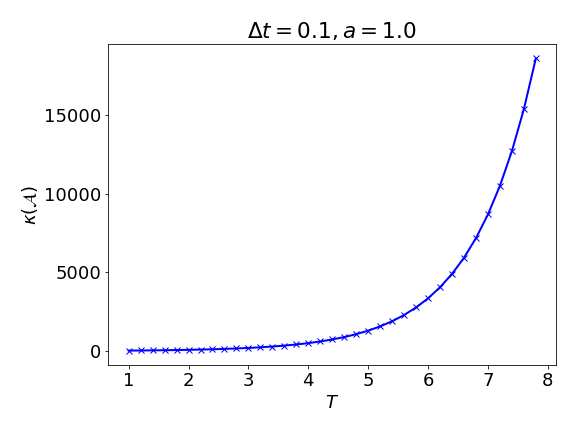
\includegraphics[width=0.4\textwidth]{ode_growth_T_a1}
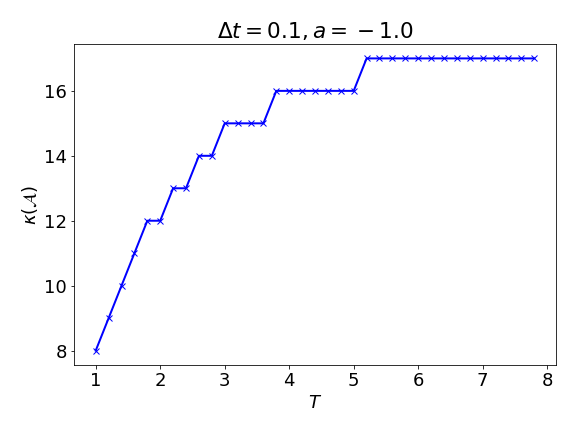
\includegraphics[width=0.4\textwidth]{ode_growth_T_am1}
\end{center}
\caption{Growth of the condition number $\kappa(\mc{A})$ with respect to $T$ with a fixed step size $\Delta t=0.1$ for $a=1.0$ and $a=-1.0$.}
\label{fig:ode_growth_T}
\end{figure}
\end{exam}


\begin{rem}
It may be tempting to modify the $(N,N)$-th entry of $\mc{A}$ to be $1+\abs{\xi}^2$ to obtain
\begin{equation}
\mc{G}=\begin{pmatrix}
1+\abs{\xi}^2 &  -\conj{\xi} & \cdots & 0 & 0\\
-\xi & 1+\abs{\xi}^2 & -\conj{\xi} & \cdots & 0 & 0\\
0 & -\xi & 1+\abs{\xi}^2 & \cdots & 0 & 0\\
\vdots & & & & &\vdots\\
0& 0 & 0 & \cdots & 1+\abs{\xi}^2 & -\conj{\xi}\\
0& 0 & 0 & \cdots & -\xi & 1+\abs{\xi}^2
\end{pmatrix}.
\end{equation}
Here  $\mc{G}$ is a Toeplitz tridiagonal matrix satisfying the requirement of \cref{prop:diag_tridiagonal}.
The eigenvalues of $\mc{G}$ take the form 
\begin{equation}
\lambda_k=1+\abs{\xi}^2+2\abs{\xi} \cos \frac{k\pi}{N+1}, \quad k=1,\ldots,N.
\end{equation}
If we take the approximation $\lambda_{\min}(\mc{A}^{\dag}\mc{A})\approx \lambda_{\min}(\mc{G})$, we would find that \cref{eqn:kappaA_scalar_ode} holds even when $\Re a>0$.
This behavior is however incorrect,  despite that the matrices $\mc{A}^{\dag}\mc{A}$ and $\mc{G}$ only differ by a single entry!
\end{rem}
% 
% 
% Note that $\mc{G}=\mc{A}^{\dag}\mc{A}+\abs{\xi}^2 e_{N,N}$ where $e_{k,l}$ is a matrix of size $N\times N$ with matrix entries $(e_{k,l})_{i,j}= \delta_{ik} \delta_{jl}$.
% Since $\abs{\xi}^2 e_{N,N}$ is positive definite, we have 
% \begin{equation}
% \norm{\mc{A}}=\sqrt{\lambda_{\max}(\mc{A}^{\dag}\mc{A})} \le \sqrt{\lambda_{\max}(\mc{G})}\le \sqrt{1+\abs{\xi}^2+2\abs{\xi}}\le 3.
% \label{eqn:A_scalar_max}
% \end{equation}
% 
% When $\Delta t $ is small, it is tempting to perform a similar approximation to estimate $\norm{A^{-1}}$. By Taylor expansion for the cosine function, we obtain
% \begin{equation}
% \begin{split}
%  \norm{\mc{A}^{-1}}^{-1}&=\sqrt{\lambda_{\min}(\mc{A}^{\dag}\mc{A})}\approx \sqrt{\lambda_{\min}(\mc{G})} \\
% &\approx  \sqrt{(1-|\xi|)^2+2\abs{\xi}\left(1-\cos(\pi \Delta t /T)\right)}\approx \Delta t \sqrt{\abs{a}^2+\frac{\pi^2}{T^2}}.
% \end{split}
% \label{eqn:A_scalar_min_false}
% \end{equation}
% Then if $\abs{a}=\Theta(1)$, we have the estimate of the condition number as $\kappa(\mc{A})=\Or\left((\Delta t) ^{-1}\right)$.
% 
% 
% 
% 
% To bound $\lambda_{\min}(\mc{A}^{\dag}\mc{A})$, we can consider 
% \begin{equation}
% \mc{G'}=\begin{pmatrix}
% 1 &  -\conj{\xi} & \cdots & 0 & 0\\
% -\xi & 1 & -\conj{\xi} & \cdots & 0 & 0\\
% 0 & -\xi & 1 & \cdots & 0 & 0\\
% \vdots & & & & &\vdots\\
% 0& 0 & 0 & \cdots & 1 & -\conj{\xi}\\
% 0& 0 & 0 & \cdots & -\xi & 1
% \end{pmatrix},
% \end{equation}
% then $\mc{G'}$ is a Toeplitz tridiagonal matrix satisfying the requirement of \cref{prop:diag_tridiagonal}.
% The eigenvalues of $\mc{G'}$ take the form 
% \begin{equation}
% \lambda_k=1+2\abs{\xi} \cos \frac{k\pi}{N+1}, \quad k=1,\ldots,N.
% \end{equation}
% Use $\abs{\xi}<1$, we have
% \begin{equation}
% \min \lambda_k\ge 1-2
% \end{equation}
% Hence
% \begin{equation}
% \lambda_{\min}(\mc{A}^{\dag}\mc{A})\ge \lambda_{\min}(\mc{G}')=\Or(\Delta t ),
% \end{equation}
% 
% 
% a similar matrix $\mc{G}_{N+1}$ of size $(N+1)\times (N+1)$. Direct calculation shows 
% \begin{equation}
% \mc{G}_{N+1}=\begin{pmatrix}
% \mc{A}^{\dag}\mc{A} & 0\\
% 0 & 0
% \end{pmatrix}
% +
% \begin{pmatrix}
% 0_{N-1} & 0 & 0\\
% 0 & |\xi|^2 & -\conj{\xi}\\
% 0 & -\xi & 1+|\xi|^2
% \end{pmatrix}
% :=\begin{pmatrix}
% 1 & 0 \\
% 0 & 0
% \end{pmatrix}
% \otimes \mc{A}^{\dag}\mc{A} + \mc{E}, 
% \end{equation}
% which satisfies the Toeplitz tridiagonal structure in \cref{prop:diag_tridiagonal}. 
% Here $\mc{E}$ is a positive definite matrix, and $0_{N-1}$ is a zero matrix of size $(N-1)\times (N-1)$. Therefore
% \begin{equation}
% \lambda_{\min}(\mc{A}^{\dag}\mc{A})\le \lambda_{\min}(\mc{G}_{N+1})=\Or(\Delta t ),
% \end{equation}
% which justifies \cref{eqn:A_scalar_min}. \LL{ However, this result is far from sharp when $a>0$.} 


\subsection{Vector case}
Here we consider a general $d>1$, but for simplicity assume $A(t)\equiv A\in\CC^{d\times d}$ is a constant matrix. We also assume $A$ is diagonalizable with eigenvalue decomposition
\begin{equation}
A=V\Lambda V^{-1},
\end{equation}
and $\Lambda=\diag(\lambda_1,\ldots,\lambda_N)$. We only consider the case $\Re \lambda_k< 0$ for all $k$.

\begin{prop}
For any diagonalizable $A\in\CC^{N\times N}$ with eigenvalue decomposition $Av_k=\lambda_k v_k$, we have
\begin{equation}
\norm{A^{-1}}^{-1}\le \min_k \abs{\lambda_k}\le \max_k \abs{\lambda_k}\le \norm{A}.
\end{equation}
\end{prop}
\begin{proof}
Use the Schur form $A=QTQ^{\dag}$, where $Q$ is an unitary matrix and $T$ is an upper triangular matrix (see e.g. \cite[Theorem 7.13]{GolubVan2013}).
The diagonal entries of $T$ encodes all eigenvalues of $A$, and the eigenvalues can appear in any order along the diagonal of $T$. The proposition follows by arranging the eigenvalue of $A$ with the smallest and largest absolute values to the $(N,N)$-th entry, respectively.
\end{proof}

The absolute stability condition of the forward Euler method requires $\Delta t \norm{A}<1$, and we are interested in the regime $\Delta t \norm{A}\ll 1$. Therefore $\Delta t \abs{\lambda_k}\ll 1$ for all $k$.


Let $I$ be an identity matrix of size $d$, and denote by $B=-(I+\Delta t A)$, then
\begin{equation}
\mc{A}^{\dag}\mc{A}=\begin{pmatrix}
I+B^{\dag}B &  B^{\dag} & \cdots & 0 & 0\\
B & I+B^{\dag}B & B^{\dag} & \cdots & 0 & 0\\
0 & B & I+B^{\dag}B & \cdots & 0 & 0\\
\vdots & & & & &\vdots\\
0& 0 & 0 & \cdots & I+B^{\dag}B & B^{\dag}\\
0& 0 & 0 & \cdots & B & I
\end{pmatrix}.
\end{equation}

Note that
\begin{equation}
\norm{B}\le \norm{I+B^{\dag}B}\le 1+(1+\Delta t \norm{A})^2\le 5.
\end{equation}
For any $\vx\in\CC^{Nd}$, 
\begin{equation}
\begin{split}
\norm{\mc{A}^{\dag}\mc{A}\vx}^2 &\le \norm{I+B^{\dag}B}\Big[(\norm{x_1}^2+\norm{x_2}^2)+(\norm{x_1}^2+\norm{x_2}^2+\norm{x_3}^2)+
\cdots\\
&+(\norm{x_{N-1}}^2+\norm{x_{N}}^2) \Big]\le 15\norm{\vx}^2.
\end{split}
\end{equation}
So $\lambda_{\max}(\mc{A}^{\dag}\mc{A})\le 15$, and 
\begin{equation}
\norm{\mc{A}}=\sqrt{\lambda_{\max}(\mc{A}^{\dag}\mc{A})}\le\sqrt{15}=\Or(1).
\end{equation}


To bound $\norm{\mc{A}^{-1}}$, we first note that from the eigenvalue decomposition of $A$, we have
\begin{equation}
\mc{A}=
\begin{pmatrix}
V \\
& V \\
& & \ddots \\
& & & V
\end{pmatrix}
\begin{pmatrix}
I & 0 & 0 & \cdots & 0 & 0\\
-(I+\Delta t \Lambda) & I & 0 & \cdots & 0 & 0\\
0 & -(I+\Delta t \Lambda) & I & \cdots & 0 & 0\\
\vdots & & & & &\vdots\\
0& 0 & 0 & \cdots & -(I+\Delta t \Lambda) & I
\end{pmatrix}
\begin{pmatrix}
V^{-1} \\
& V^{-1} \\
& & \ddots \\
& & & V^{-1}
\end{pmatrix}.
\end{equation}
Hence
\begin{equation}
\norm{\mc{A}^{-1}}\le \norm{V}\norm{V^{-1}}\max_{k} \norm{\mc{A}_k^{-1}}=\kappa(V) \norm{\mc{A}_k^{-1}}.
\end{equation}
Here $\kappa(V)=\norm{V}\norm{V^{-1}}$ is the condition number of the eigenvector matrix
\begin{equation}
\mc{A}_k=\begin{pmatrix}
1 & 0 & 0 & \cdots & 0 & 0\\
-(1+\Delta t \lambda_k) & 1 & 0 & \cdots & 0 & 0\\
0 & -(1+\Delta t \lambda_k) & 1 & \cdots & 0 & 0\\
\vdots & & & & &\vdots\\
0& 0 & 0 & \cdots & -(1+\Delta t \lambda_k) & 1
\end{pmatrix}.
\end{equation}
This reduces the problem to the scalar case.
Let $\xi_k=1+\Delta t \lambda_k$, and assume
\begin{equation}
\Re \lambda_k <0, \quad \Delta t\abs{\lambda_k}<(-\Re \lambda_k)/\abs{\lambda_k}, \quad \forall k.
\end{equation}
Then from \cref{eqn:A_scalar_min} we have
\begin{equation}
 \min_{k}\norm{\mc{A}^{-1}_k}^{-1}\ge \frac{\Delta t \min_{k}(-\Re \lambda_k)}{2}.
 \end{equation}
So if $\min_{k}(-\Re \lambda_k)=\Theta(1)$, we have 
\begin{equation}
\kappa(\mc{A})=\Or(\kappa(V)/\Delta t),
\end{equation}
and the cost of the HHL algorithm is $\Or((\Delta t)^{-2}\epsilon^{-2}\kappa(V))$.
Hence compared to the scalar case, the condition number of the eigenvector matrix $V$ can play an important role. 

% We may add $B^{\dag}B$ to the bottom-right block to make it a block Toeplitz tridiagonal matrix, and obtain a modified matrix
% \begin{equation}
% \mc{G}=\begin{pmatrix}
% I+B^{\dag}B &  B^{\dag} & \cdots & 0 & 0\\
% B & I+B^{\dag}B & B^{\dag} & \cdots & 0 & 0\\
% 0 & B & I+B^{\dag}B & \cdots & 0 & 0\\
% \vdots & & & & &\vdots\\
% 0& 0 & 0 & \cdots & I+B^{\dag}B & B^{\dag}\\
% 0& 0 & 0 & \cdots & B & I+B^{\dag}B
% \end{pmatrix}.
% \end{equation}
% This modification can be similarly justified as in the scalar case.
% 

\subsection{Computing observables}

The solution of \cref{eqn:qlsp_ode} means that the normalized state $\ket{\vx}$ is computed to precision $\epsilon$ and stored in the quantum computer.
In order to evaluate observables at the final time $T$, i.e., $\braket{x(T)|O|x(T)}$, we find that by the normalization condition, $\norm{x(T)}$ is on average $\Or(N^{-\frac12})=\Or((\Delta t)^{\frac12})$, and $\braket{x(T)|O|x(T)}=\Or(\Delta t)$. 
Therefore instead of reaching accuracy $\epsilon$, the Monte Carlo procedure must reach precision $\Or(\epsilon\Delta t)$. 
This increases the number of samples by another factor of $\Or((\Delta t)^{-2})$.

There is however a simple way to overcome this problem.
Instead of solving \cref{eqn:qlsp_ode}, we can redefine $\vx$ by artificially padding the vector with $N$ copies of the final state $x_N$. This can be written as
and can be reinterpreted as
\begin{equation}
\vX=\ket{0}\otimes \vx+\ket{1} \otimes \vy,
\end{equation}
with the unnormalized vector
\begin{equation}
\vx=\begin{pmatrix}
x_1\\
x_2\\
\vdots\\
x_{N}
\end{pmatrix},
\quad
\vy=\begin{pmatrix}
x_{N+1}\\
x_{N+2}\\
\vdots\\
x_{2N}
\end{pmatrix}=\begin{pmatrix}
x_{N}\\
x_{N}\\
\vdots\\
x_{N}
\end{pmatrix},
\end{equation}
and the corresponding linear systems of equation becomes
\begin{equation}
\begin{pmatrix}
I & \\
-(I+\Delta t A_1) & I \\
& & &\ddots\\
&  & & -(I+\Delta t A_{N-1}) & I\\
&&&&-I & I\\
&&&& &  -I& I \\
&&&& &  & & \ddots\\
&&&&&&&-I & I
\end{pmatrix}
\begin{pmatrix}
x_1\\
x_2\\
\vdots\\
x_{N}\\
x_{N+1}\\
x_{N+2}\\
\vdots\\
x_{2N}
\end{pmatrix}
=
\begin{pmatrix}
(I+\Delta t A_0)x_0+\Delta t b_0\\
\Delta t b_1\\
\vdots\\
\Delta t b_{N-1}\\
0\\
0\\
\vdots\\
0
\end{pmatrix}.
\label{eqn:modify_qsp_ode}
\end{equation}
Note that the solution vector only requires one ancilla qubit, after solving the equation
The condition number of this modified equation is still $\kappa=\Or((\Delta t)^{-1})$, so the total query complexity is $\Or((\Delta t)^{-2}\epsilon^{-2})$. 
By solving the modified equation \cref{eqn:modify_qsp_ode} to precision $\epsilon$, we can estimate $\braket{x(T)|O|x(T)}$ by
\begin{equation}
\braket{\vy|I\otimes O|\vy}
\end{equation}
of which the magnitude does not scale with $\Delta t$. 
Here $I$ is the identity matrix of size $N$, and $\vy$ can be obtained by measuring the ancilla qubit and obtain $1$. 
If the norm of $\norm{x(t)}$ is comparable for all $t\in[0,T]$, then the success probability will be $\Theta(1)$ after $\ket{\vX}$ is obtained.



\section{Example: Solve the heat equation*}\label{sec:heatequation}

As an application of the differential equation solver in \ref{sec:linear_ode}, let us consider a toy problem of solving the heat equation in one-dimension with Dirichlet boundary conditions
\begin{equation}
\partial_t u(r,t)=u''(r), \quad r\in \Omega=[0,1], \quad u(0,t)=u(1,t)=0.
\end{equation}
After spatial discretization using the central finite difference method with $d$ grid points, this becomes a linear ODE system
\begin{equation}
\partial_t u=-Au,
\end{equation}
where $A\in \RR^{N\times N}$ is a tridiagonal matrix given by \cref{eqn:A_tridiagonal}.
After applying the forward Euler method and discretize the simulation time $T$ into $L$ intervals with $\Delta t=T/L$, we obtain a linear system of size $NL$. The eigenvalues of $-A$, denoted by $\lambda_k$, are all negative and satisfy
\begin{equation}
-\frac{4}{h^2}\approx -\norm{A}\le \lambda_k\le -\norm{A^{-1}}^{-1}\approx -\frac{1}{\pi^2}.
\end{equation}The absolute stability condition requires $\abs{1+\Delta t \lambda_k}<1$, or $\Delta t<h^2/4=\Or(N^{-2})$, which implies $L=\Or(N^2)$.   Since $A$ is Hermitian, we have $\kappa(V)=1$. 
So for $T=\Or(1)$, the query complexity for solving the heat equation is $\Or(N^2\epsilon^{-2})$, which is the same as solving Poisson's equation.

Again, the potential advantage of the quantum solver only appears when solving the $d$-dimensional heat equation
\begin{equation}
\partial_t u(\vr,t)=\Delta u(r), \quad r\in \Omega=[0,1]^d, \quad u(\cdot,t)|_{\partial \Omega}=0.
\end{equation}
This can be written as a linear system of equations
\begin{equation}
\partial_t u=-\mc{A} u, 
\end{equation}
where $\mc{A}$ is given in \cref{eqn:A_ddimension}. 
The eigenvalues of $\mc{A}$ are all negative.
Note that $\norm{\mc{A}}=\Theta(dN^2)$, then $h=\Or(d^{-1}N^{-2})$, and the query complexity of the HHL solver is $\Or(dN^2 \epsilon^{-2})$.
This could potentially have an exponential advantage over classical solvers.

\vspace{2em}

\begin{exer}[Quantum counting] Given query access to a function $f:\{0,1\}^N \rightarrow \{0,1\}$ design a quantum algorithm that computes the size of its kernel, i.e.,, total number of $x$'s that satisfy $f(x)=1$. 
\end{exer}


\begin{exer}
Consider the initial value problem of the linear differential equation~\cref{eqn:linear_ode}. 
\begin{enumerate}
    \item Construct the linear system of equations 
    \[
    \bvec{\mathcal{A}} \vx = \vb
    \]
    like \cref{eqn:qlsp_ode} using the backward Euler method.
    \item In the scalar case when $A(t) \equiv a \in \mathbb{C}$ is a constant satisfying $\Re(a) \leq 0$, estimate the query complexity of the HHL algorithm applying to the linear system constructed in (1).
\end{enumerate}
\end{exer}
